%----------------------------------------------------------------------------
\chapter{Szöveges PSC leíró nyelv kibővítése}
%----------------------------------------------------------------------------

A szakdolgozatom során készített szöveges \textit{PSC} leíró nyelvet \cite{Bakai} az \textit{Xtext} technológia segítségével definiáltam.
A nyelv fő elemei:
\begin{itemize}
    \item objektumok (az üzenetekkel kommunikáló rendszerkomponensek)
    \item üzenetek
    \item megkötések
    \item szcenárió
    \item \textit{alt} operátor
    \item \textit{loop} operátor
    \item \textit{par} operátor
\end{itemize}

A nyelvben egy objektumot az „\textit{object}” kulcsszóval lehet bevezetni.
Meg kell adni az objektum típusát és a nevét, ezután a definíciót egy ’;’-vel lehet lezárni.
Megkötések specifikálásához a „\textit{constraint}” kulcsszót kell használni.
Elég csupán a megkötés nevét megadni és '\{' '\}' jelek közt, a megkötéshez tartozó üzeneteket.

Egy sima üzenet megadásához a „\textit{message}” kulcsszó szükséges.
A „\textit{message}” kulcsszó előtt lévő „\textit{fail}” vagy „\textit{required}” kulcssavakkal adhatunk meg nem kívánt vagy elvárt üzeneteket.
A „\textit{strict}” kulcsszóval adhatjuk meg, hogy az üzenet sorrendje megkötött.
Az üzenet küldőjét és fogadóját „\textit{<küldő> -> <fogadó>}” formában jelezzük.
Múltbéli vagy jövőbeli megkötéseket a \textit{pastConstraint} vagy \textit{futureConstraint} kulcsszavakkal adhatunk meg.
A kulcsszó után, '\{' '\}' jelek közt adhatjuk meg, hogy melyik előzőleg definiált megkötést helyezzük el az üzeneten.
Egy üzenet definíció végére szükséges ’;’-őt tenni, így elválasztjuk a többi üzenettől.

A nyelvet két új elemmel bővítettem ki:
\begin{itemize}
    \item időzített feltétel
    \item óraváltozó nullázása
\end{itemize}
Az új nyelvi elemek bevezetéséhez az eredeti üzenet leíró \textit{Xtext} szabályt (\textit{Message}) kellett kibővíteni.
A kibővített nyelvtani szabályt a \ref{minotor_message} kódrészlet tartalmazza.
Az eredeti nyelvtani szabályt a \ref{minotor_message_original} kódrészlet tartalmazza.
Bevezettem egy új \textit{clockConstraint} kulcsszót, amivel egy időzítési feltételt lehet megadni.
Ezt a \textit{cConstraint} változóban tárolom.
A \textit{resetClock} attribútum tárolja a visszaállítandó óraváltozó nevét.
A teljes nyelvtan definíció megtekinthető a \textit{Függelékben} (\ref{xtext_tpsc_grammar}).

\begin{lstlisting}[language=java, frame=single, float=ht!, caption={Eredeti \textit{Message} nyelvtani szabály \cite{Bakai}.},captionpos=b,label=minotor_message_original]
Message:
    'message' name=Name (required?='required')? (fail?='fail')? (strict?='strict')?
    sender=[Object] '->' receiver=[Object]
    (past?='past')? (future?='future')? (constraint?='constraint')?
    ('{')? (c=[Constraint])? ('}')? ';'

;
\end{lstlisting}

\begin{lstlisting}[language=java, frame=single, float=ht!, caption={Kibővített \textit{Message} nyelvtani szabály.},captionpos=b,label=minotor_message]
Message:
	LooseMessage | StrictMessage | PastMessage | FutureMessage | StrictFutureMessage
	| RequiredLooseMessage | RequiredStrictMessage | RequiredPastMessage | RequiredFutureMessage | RequiredStrictFutureMessage
	| FailMessage | FailStrictMessage | FailPastMessage
;

LooseMessage:
	'message' name=ID '(' (params+=Params | constantparams+=ConstantParams) ')'
	sender=[Object] '->' receiver=[Object]
	('clockConstraint' '{' cConstraint=ClockConstraintExpression '}')? 
	(resetclock=ResetClock)? ';'
;
\end{lstlisting}

\begin{figure}[!ht]
    \centering
    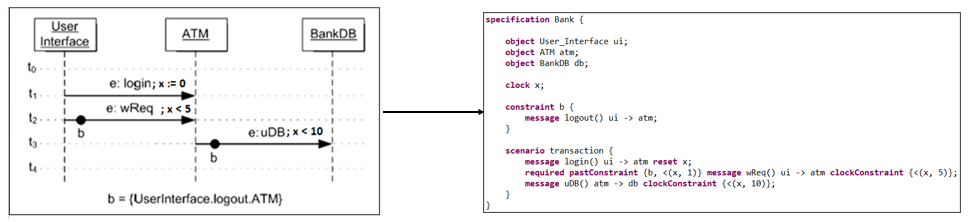
\includegraphics[width=150mm, keepaspectratio]{figures/11abra.png}
    \caption{\textit{TPSC} diagramból szöveges leírás az \textit{Xtext} nyelv használatával.}
    \label{xtext_language_example}
\end{figure}

A \ref{xtext_language_example} ábrán látható, hogy egy \textit{TPSC} diagramot hogyan tudunk leírni a nyelvünk segítségével.
Definiálhatjuk a diagramban szereplő objektumokat, a megkötéseket amiket használni fogunk és végül, hogy milyen üzenetek vannak a követelményünkben.

\begin{figure}[!ht]
    \centering
    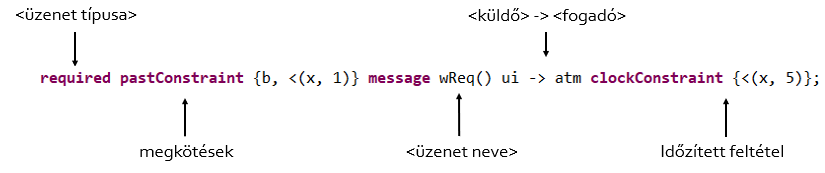
\includegraphics[width=150mm, keepaspectratio]{figures/12abra.png}
    \caption{Egy \textit{TPSC} üzenet felépítése a definiált \textit{Xtext} nyelvben.}
    \label{xtext_message}
\end{figure}

A \ref{xtext_message} ábrán látszik, hogy megjelenik a \textit{clockConstraint} kulcsszó ami egy időzítési feltétel megadására szolgál.
A kulcsszó után kapcsos zárójelek közt megadható a feltétel.
Egy időzítési feltételt egy adott óraváltozóra adhatunk meg.
Négy operátort definiál ehhez a nyelv:
\begin{itemize}
    \item < (kisebb)
    \item > (nagyobb)
    \item <= (kisebb egyenlő)
    \item >= (nagyobb egyenlő)
\end{itemize}
Az operátor után ’(’ ’)’ jelek között adható meg az óraváltozó, majd utána az érték.
Például a \textit{<(x, 5)} kifejezés azt jelenti, hogy az \textit{x} óraváltozóban lévő időértéknek kisebbnek kell lennie öt időegységnél.

Időzítési feltételt egy megkötésre is megadhatunk, '\{' '\}' jelek között, ’,’-vel elválasztva a megkötés után.
A \textit{reset} kulcsszó az óraváltozó nullázására szolgál.